%%%%%%%%%%%%%%%%%%% Especificación:
\begin{frame}[fragile]{Definiciones:}{Vector Tiempo.}
  \justifying
  \textbf{Sistema Vectorial de Relojes.} Es un mecanismo
  capaz de caracterizar estados locales (en adelante, eventos)
  en un sistema distribuido, asociando un valor vectorial
  a cada estado.\\[0.3cm]
  %  Esto nos permite saber que relación hay entre estos estados.
  
  \textbf{Tiempo Vectorial.} Es la noción de tiempo capturada
  por los relojes vectoriales.\\[0.3cm]

  \textbf{Caracterización Formal del Tiempo Vectorial.} Sea
  \code{date(e)} la caracterización asociada a un evento \code{e},
  de tal manera que se cumple:
  \begin{enumerate}
  \item $\forall_{e_1, e_2}:\left(e_1 \rightarrow e_2\right)
    \Leftrightarrow \code{date($e_1$)} < \code{date($e_2$)}$.
  \item $\forall_{e_1, e_2}: \left(e_1\ ||\ e_2\right) \Leftrightarrow
    \code{date($e_1$)}\ ||\ \code{date($e_2$)}$.
  \end{enumerate}
  \begin{figure}
    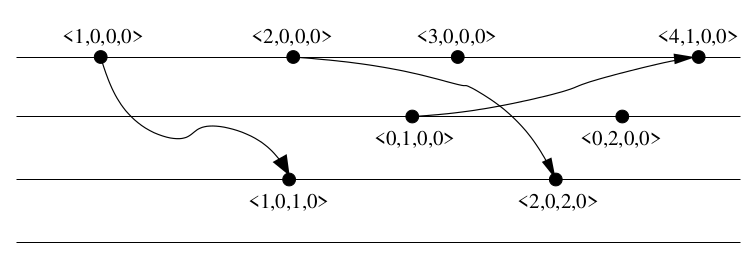
\includegraphics[height = 2.5cm]{./Imagenes/RelojVectorialSimple.png}
    \caption{Reloj Vectorial con tiempos locales.}
  \end{figure}
\end{frame}
